\documentclass[oneside,final,14pt]{extreport}

%% my command
%%%%%%%%%%%%%%
% Путь к файлу с изображениями
\newcommand{\picPath}{pictures}
% Величина отступа
\newcommand{\indentSpace}{1.25cm}
% Сокращения
\newcommand{\urlTitle}{ $-$ URL: }
%%%%%%%%%%%%%%%


% Изменяем шрифт
\usepackage{fontspec}
\setmainfont{Times New Roman}
\listfiles

% Полуторный интервал
\linespread{1.6}

% Отступ
\setlength\parindent{\indentSpace}

% Математика
\usepackage{mathtools}


% Картинки
\usepackage{graphicx}
\usepackage{subcaption}

% Языковой пакет
\usepackage[russianb]{babel}

% Таблицы
\usepackage{tabularx}

% Настройка подписей к фигурам
% Меняем заголовки картинок
\usepackage[ labelsep= endash]{caption}
\captionsetup{%
   figurename= Рисунок,
   tablename= Таблица,
   justification= centering% Формат - по центру
}         

% Кирилица в подфигурах
\renewcommand{\thesubfigure}{\asbuk{subfigure}}
% разделитель в подфигурах - правая скобка
\DeclareCaptionLabelSeparator{r_paranthesis}{)\quad }
\captionsetup[subfigure]{labelformat=simple, labelsep=r_paranthesis}

% Добавляем итератор \asbuk,
% чтобы использовать кирилицу
% как маркеры
\usepackage{enumitem}
\makeatletter
\AddEnumerateCounter{\asbuk}{\russian@alph}{щ}
\makeatother

% Меняем маркеры в перечислениях
% Списки уровня 1
\setlist[enumerate,1]{label=\arabic*),ref=\arabic*}
% Списки уровня 2
\setlist[enumerate,2]{label=\asbuk*),ref=\asbuk*}
% Перечисления
\setlist[itemize,1]{label=$-$}
% Удаляем отступы перед и после
% списка
\setlist[itemize]{noitemsep, topsep=0pt}
\setlist[enumerate]{noitemsep, topsep=0pt}

% Красная строка в начале главы
\usepackage{indentfirst}

% Убиваем перенос
\usepackage[none]{hyphenat}

% Перенос длинных ссылок
\usepackage[hyphens]{url}
\urlstyle{same}

% Выравнивание по ширине
\usepackage{microtype}

%\usepackage[fontfamily=courier]{fancyvrb}
%\usepackage{verbatim}%     configurable verbatim
% \makeatletter
%  \def\verbatim@font{\normalfont\sffamily% select the font
%                     \let\do\do@noligs
%                     \verbatim@nolig@list}
%\makeatother

% Границы
\usepackage{vmargin}
\setpapersize{A4}
% отступы
%\setmarginsrb 
%{3cm} % левый
%{2cm} % верхний
%{1cm} % Правый
%{2cm} % Нижний
%{0pt}{0mm} % Высота - отступ верхнего колонтитула
%{0pt}{0mm} % Высота - отступ нижнего  колонтитула

\setlength\hoffset{0cm}
\setlength\voffset{0cm}
\usepackage[top=2cm, bottom=2cm, left=3cm, right=2cm,
]{geometry}
 		
% Настройка заглавиий
\addto\captionsrussian{% Replace "english" with the language you use
  \renewcommand{\contentsname}% содержания
    {\hfill\bfseries
    СОДЕРЖАНИЕ
	\hfill    
    }%
   \renewcommand{\bibname}% списка источников
    {\hfill\bfseries
    	СПИСОК ИСПОЛЬЗОВАННЫХ ИСТОЧНИКОВ
	\hfill
	}% 
}%\

%\renewcommand{\contentsname}{\hfill\bfseries СОДЕРЖАНИЕ \hfill} 

% Настройка  заглавий в главах
\usepackage{titlesec}


%\titleformat
%{\chapter} % command
%[display]
%{
%\bfseries
%} % format
%{
%\thechapter.
%} 	% label
%{ 
%	0 pt
%} % sep
%{    
%\centering
%} % before-code

\titleformat{\chapter}
            {\bfseries}
            {\hspace{\indentSpace}\thechapter\hspace{1em}}
            {0pt}
            {
            \vspace{0mm} }
            [\vspace{14pt}]% Отступ после
% Начальный сдвиг заголовка 50 pt = 1.763888888cm.
% Второй параметр- сдвиг до = 2cm - 50pt
\titlespacing{\chapter}{0pt}{-0.2361cm}{0pt}

\titleformat{\section}
{\bfseries}{\hspace{\indentSpace}\thesection}{1em}{}

\titleformat{\subsection}
{\bfseries}{\hspace{\indentSpace}\thesubsection}{1em}{}

%\titleformat{\section}
%            {\bfseries}
%            {\thechapter.\hspace{1em}}
%            {0pt}
%            {\centering
%            \vspace{0mm} }
%            [\vspace{14pt}]% Отступ после
%\titlespacing{\section}{0pt}{-50pt}{0pt}

% Конец настройка заглавий

% Форматирование списка источников
\makeatletter
\renewcommand*{\@biblabel}[1]{\hfill#1}
\makeatother

% Убрать отсупы в списке источников
\usepackage{lipsum}

% ADD THE FOLLOWING COUPLE LINES INTO YOUR PREAMBLE
\let\OLDthebibliography\thebibliography
\renewcommand\thebibliography[1]{
  \OLDthebibliography{#1}
  \setlength{\parskip}{0pt}
  \setlength{\itemsep}{0pt plus 0.3ex}
}



% Добавить точки в оглавление
\usepackage{tocstyle}
\newcommand{\autodot}{.}


% Чтобы картинки вставляись
% куда надо
\usepackage{float}

% Для вычисления кол-ва страниц
\usepackage{lastpage}

% Для вычисления кол-ва рисунков и таблиц
%%%
\usepackage{etoolbox}

\newcounter{totfigures}
\newcounter{tottables}

\providecommand\totfig{} 
\providecommand\tottab{}

\makeatletter
\AtEndDocument{%
  \addtocounter{totfigures}{\value{figure}}%
  \addtocounter{tottables}{\value{table}}%
  \immediate\write\@mainaux{%
    \string\gdef\string\totfig{\number\value{totfigures}}%
    \string\gdef\string\tottab{\number\value{tottables}}%
  }%
}
\makeatother

\pretocmd{\chapter}{\addtocounter{totfigures}{\value{figure}}\setcounter{figure}{0}}{}{}
\pretocmd{\chapter}{\addtocounter{tottables}{\value{table}}\setcounter{table}{0}}{}{}
%%%

% Режим релиза
\sloppy
\usepackage{layout}

\begin{document}
\tableofcontents
\newpage
\begin{center}
\bfseries ВВЕДЕНИЕ
\end{center}
\addcontentsline{toc}{chapter}{Введение}

	На сегодняшний день многие дети перестали верить в Деда Мороза. Компьютерные игры и социальные сети отнимают все время молодых людей, делая их зависимыми от компьютера. Зависимость развилась настолько сильно, что дети разучились читать книжки, а тем более писать вручную. Специально для таких детей разработан сайт Дедушки Мороза ФКТиПМ. Чтобы отправить ему письмо, совершенно не нужно быть грамотным. Единственное требование к пользователю - умение читать и кликать мышью. Кроме того, ответ от Деда Мороза приходит мгновенно, не требуя ждать пользователя пару месяцев как в случае бумажных писем. Дедушка Мороз ФКТ и ПМ подберёт для каждого ребенка тот подарок, которого он заслуживает.
	
	Целью работы является изучение связки php-html-css-javascript и увеличение новогоднего настроения среди населения. 
	
	World Wide Web – глобальная компьютерная сеть, на сегодняшний день содержит миллионы сайтов, на которых размещена всевозможная информация. Люди получают доступ к этой информации посредством использования технологий Internet. Для поиска по интернету используют специальные программы – Web-браузеры, которые существенно облегчают путешествие по бескрайним просторам интернета   
\chapter{Обзор трёхзвенной структуры}
Как правило компьютеры и программы, входящие в состав информационной системы, не являются равноправными. Некоторые из них владеют ресурсами (файловая система, процессор, принтер, база данных и т.д.), другие имеют возможность обращаться к этим ресурсам. Компьютер (или программу), управляющий ресурсом, называют сервером этого ресурса (файл-сервер, сервер базы данных, вычислительный сервер). Клиент и сервер какого-либо ресурса могут находится как на одном компьютере, так и на различных компьютерах, связанных сетью.

В рамках многоуровневого представления вычислительных систем можно выделить три группы функций, ориентированных на решение различных подзадач: 

\begin{itemize}
\item функции ввода и отображения данных (обеспечивают взаимодействие с пользователем);
\item прикладные функции, характерные для данной предметной области;
\item функции управления ресурсами (файловой системой, базой данных и т.д.).
\end{itemize}

Выполнение этих функций в основном обеспечивается программными средствами, которые можно представить в виде взаимосвязанных компонентов, где:
\begin{itemize}
\item компонент представления отвечает за пользовательский интерфейс;
\item прикладной компонент реализует алгоритм решения конкретной задачи;
\item компонент управления ресурсом обеспечивает доступ к необходимым ресурсам.
\end{itemize}

Автономная система (компьютер, не подключенный к сети) представляет все эти компоненты как на различных уровнях (ОС, служебное ПО и утилиты, прикладное ПО), так и на уровне приложений (не характерно для современных программ). Так же и сеть — она представляет все эти компоненты, но, в общем случае, распределенные между узлами. Задача сводится к обеспечению сетевого взаимодействия между этими компонентами.

Архитектура «клиент-сервер» определяет общие принципы организации взаимодействия в сети, где имеются серверы, узлы-поставщики некоторых специфичных функций (сервисов) и клиенты, потребители этих функций.

Практические реализации такой архитектуры называются клиент-серверными технологиями. Каждая технология определяет собственные или использует имеющиеся правила взаимодействия между клиентом и сервером, которые называются протоколом обмена (протоколом взаимодействия).

Тенденция в клиент-серверных технологиях связана со все большим использованием распределенных вычислений. Они реализуются на основе модели сервера приложений, где сетевое приложение разделено на две и более частей, каждая из которых может выполняться на отдельном компьютере. Выделенные части приложения взаимодействуют друг с другом, обмениваясь сообщениями в заранее согласованном формате. В этом случае двухзвенная клиент-серверная архитектура становится трехзвенной (three-tier, 3-tier).

Как правило, третьим звеном в трехзвенной архитектуре становится сервер приложений, т.е. компоненты распределяются следующим образом:
-представление данных — на стороне клиента.
-прикладной компонент — на выделенном сервере приложений (как вариант, выполняющем функции промежуточного ПО).
-управление ресурсами — на сервере БД, который и представляет запрашиваемые данные.

О преимуществах трехзвенной структуры в сравнении с двухзвенной можно узнать \cite{bib:habr},
Трехзвенная архитектура может быть расширена до многозвенной (N-tier, Multi-tier) путем выделения дополнительных серверов, каждый из которых будет представлять собственные сервисы и пользоваться услугами прочих серверов разного уровня\cite{bib:meth}.

\chapter{Актуальность разработки сайтов}
Несмотря на то, что интернет давно и прочно вошел в нашу жизнь, многие предприниматели и даже крупные фирмы не понимают, что им даст создание собственного сайта, ведь есть другие хорошо зарекомендовавшие себя проверенные способы саморекламы: телевидение, радио, СМИ, баннеры, флайеры и тому подобное.

У любой современной компании существует сайт. Это один из элементов престижа, ведь именно в Интернете потенциальные клиенты будут в первую очередь искать информацию о фирме. И если у нее нет хотя бы одностраничника с прайсом, это покажется подозрительным – насколько же это неуспешная фирма, если не может даже небольшой веб-ресурс создать?

Актуальность создания сайта состоит также в том, что если вы хотите донести информацию максимально быстро до огромного количества людей, то лучше, чем с помощью собственного сайта сделать это не получится никак. Веб-ресурс позволяет представить информацию о компании и ее товарах или услугах сжато и одновременно полноценно. Также сайт может сообщать о новостях фирмы, об изменениях в прайсе или режиме работы, содержать отзывы благодарных клиентов.

Совсем не каждая фирма нуждается в крупном портале со сложным дизайном и функционалом. Иногда бывает достаточно небольшого сайта-визитки, который можно сделать самостоятельно или же заказать профессионалам за небольшую плату.

Необходимо понимать, что ни один другой ресурс не даст столько преимуществ, сколько собственный сайт, будь это визитка, Интернет-магазин или любой другой веб-ресурс.

Нужно отметить, что одним только созданием сайта дело не ограничится. Его будет необходимо развивать и поддерживать, увеличивать конверсию и своевременно пополнять, а это задача не из легких. Однако все эти усилия и затраты сполна окупятся прибылями, которые принесет сайт.

Вы можете попробовать сделать сайт самостоятельно, но вскоре поймете, что поддержка и наполнение сайта требуют много времени, сил и специфических навыков. Доверьте свой веб-ресурс профессионалам Cetera Labs, и ваш сайт окажется в надежных руках команды профессионалов.

\chapter{Структура сайта}

Сайт состоит из главной страницы и страницы ответа деда мороза. В первую очередь сайт делится на две равнозначные, но всё же разные части: back-end и front-end \cite{bib:Sinica}. Средства для тех. реализации проекта (HTML, CSS, JS, PHP) были выбраны как наиболее распространённые и доступные. К тому же именно их нам необходимо изучить в рамках данного курса сетевых технологий.

\section{Front-end сайта}

Обе страницы сайда  Деда Мороза ФКТиПМ  объединены единым лаконичным стилем, который сразу увеличивает новогоднее настроение в разы. Страницы сайта написаны на языке разметки html \cite{bib:html}  с пользованием стилей css \cite{bib:css}. На главной странице (рисунок \ref{site:letter}) можно видеть форму в виде письма. В эту форму необходимо ввести свои личные данные: имя, возраст и город, чтобы Дедушка мороз мог разыскать ребенка в случае, когда это необходимо . Ниже идет список из десяти пожеланий, которые ребенок хотел бы отправить Деду Морозу (рисунок \ref{site:wishes}). Желания хранятся в базе данных и подгружаются автоматически. Администратор сайта (Дед Мороз ФКТиПМ) может добавлять список возможных пожеланий через командную строку. Внизу находится строка с текстом пожелания и большая кнопка для отправки письма.
\begin{figure}[H]
  \centering
  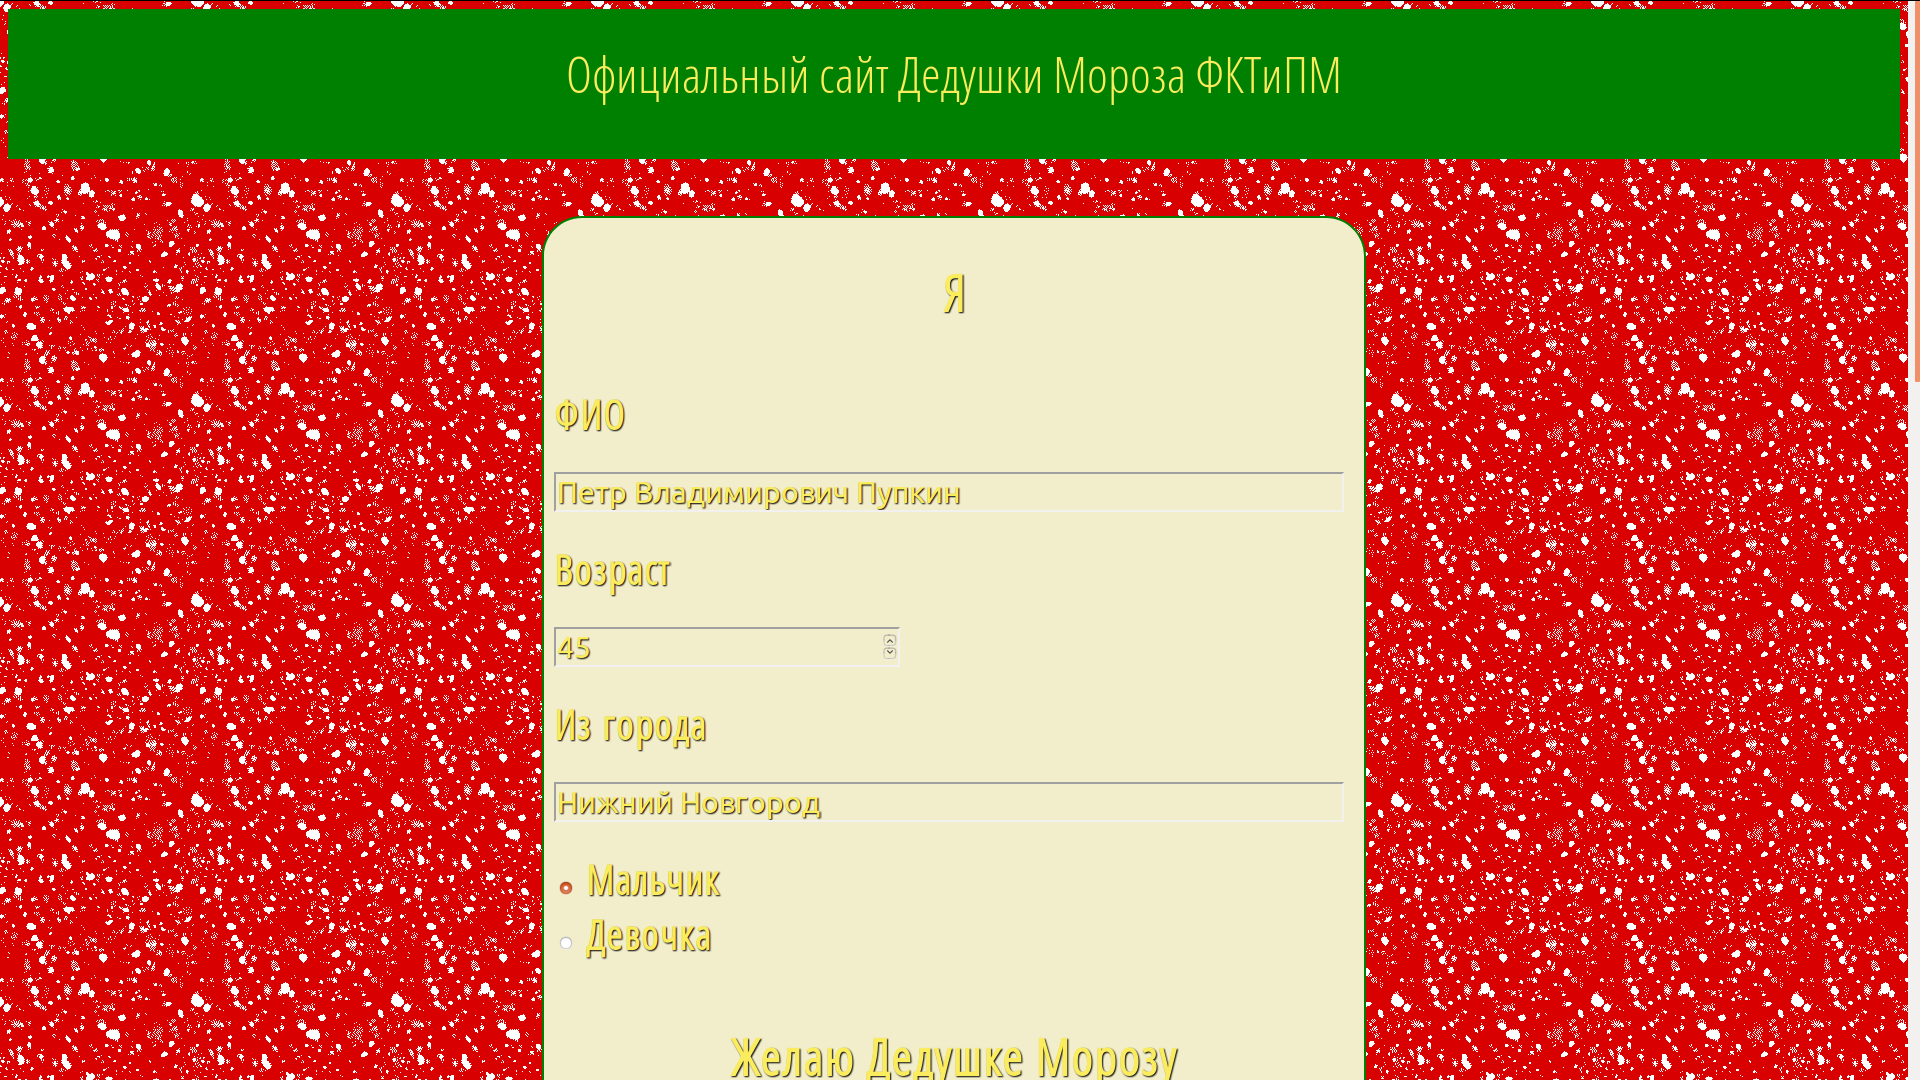
\includegraphics[width=\linewidth]{\picPath/head.png}
  \caption{ главная страница сайта }
  \label{site:letter}
\end{figure}

\begin{figure}[H]
	\centering
	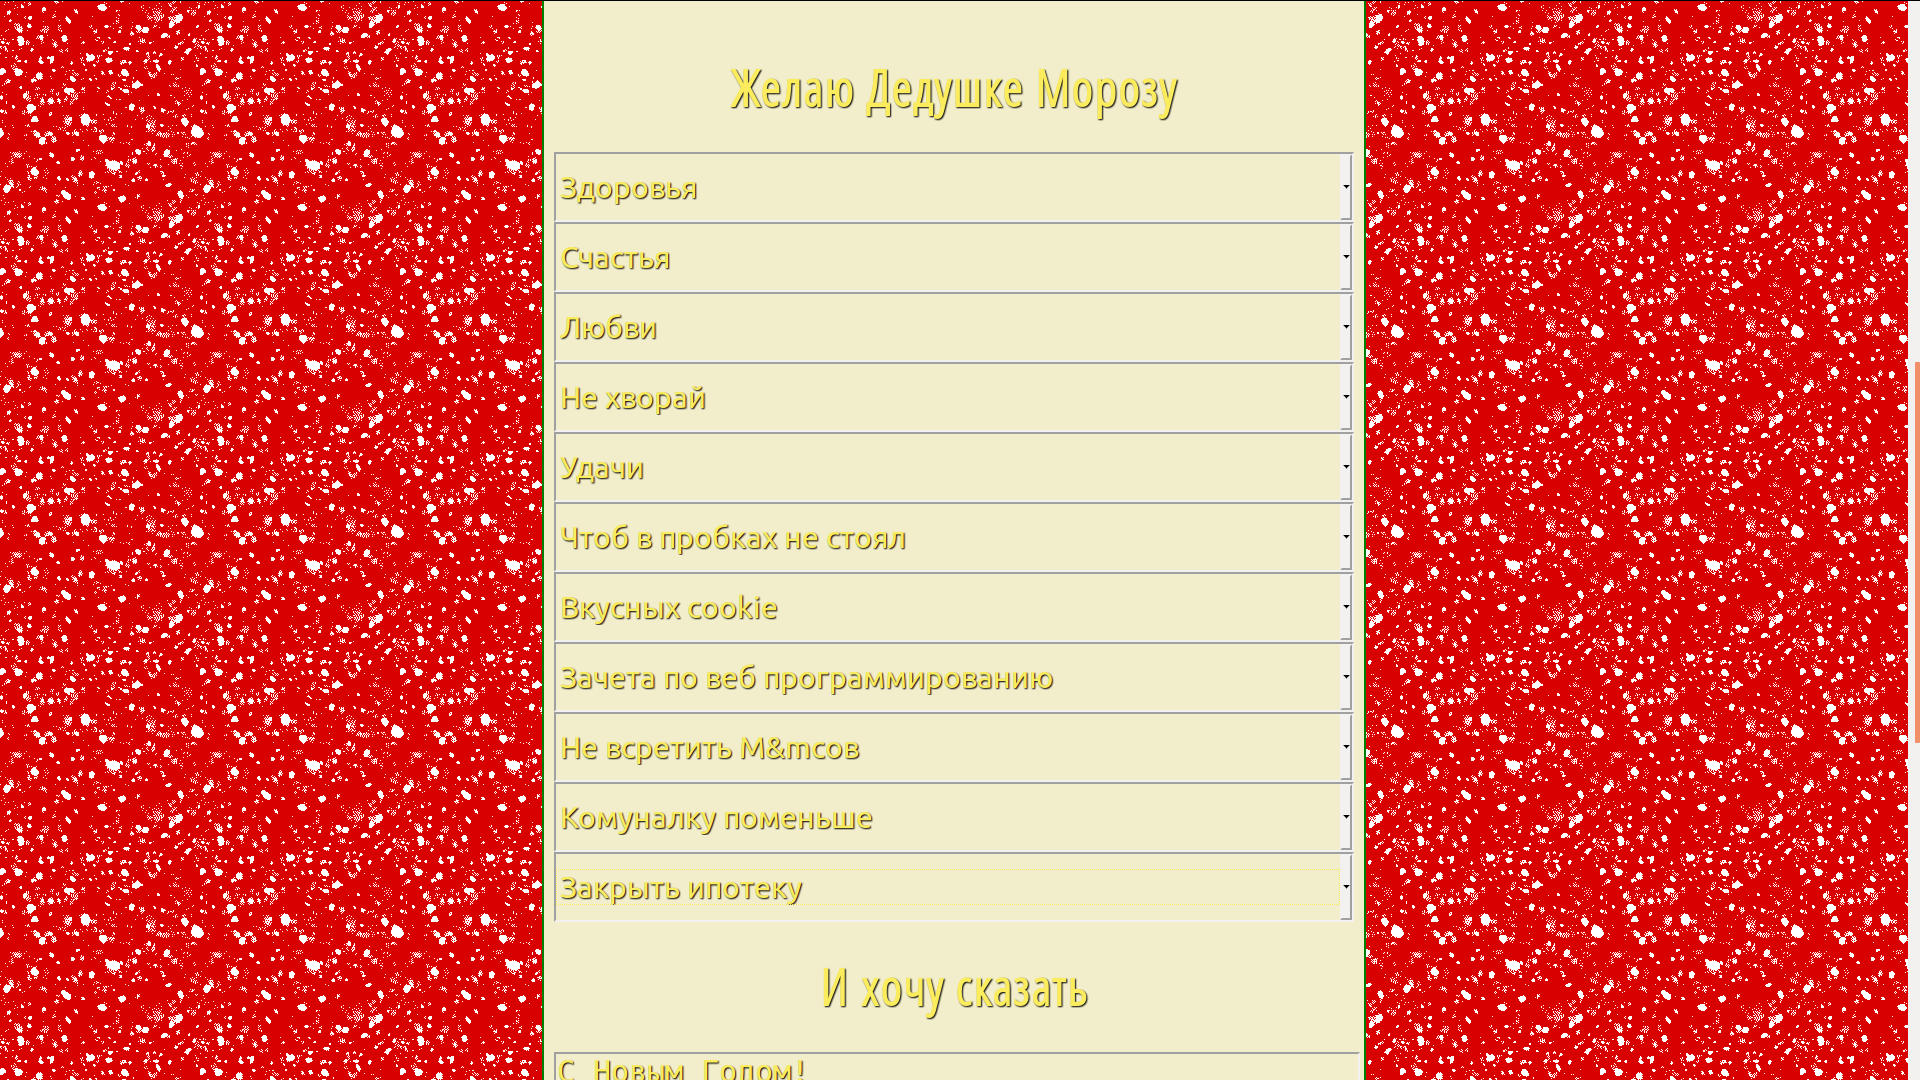
\includegraphics[width=\linewidth]{\picPath/wishes.png}
	\caption{ список пожеланий для Дедушки Мороза }
  	\label{site:wishes}
\end{figure}

\begin{figure}[H]
	\centering
	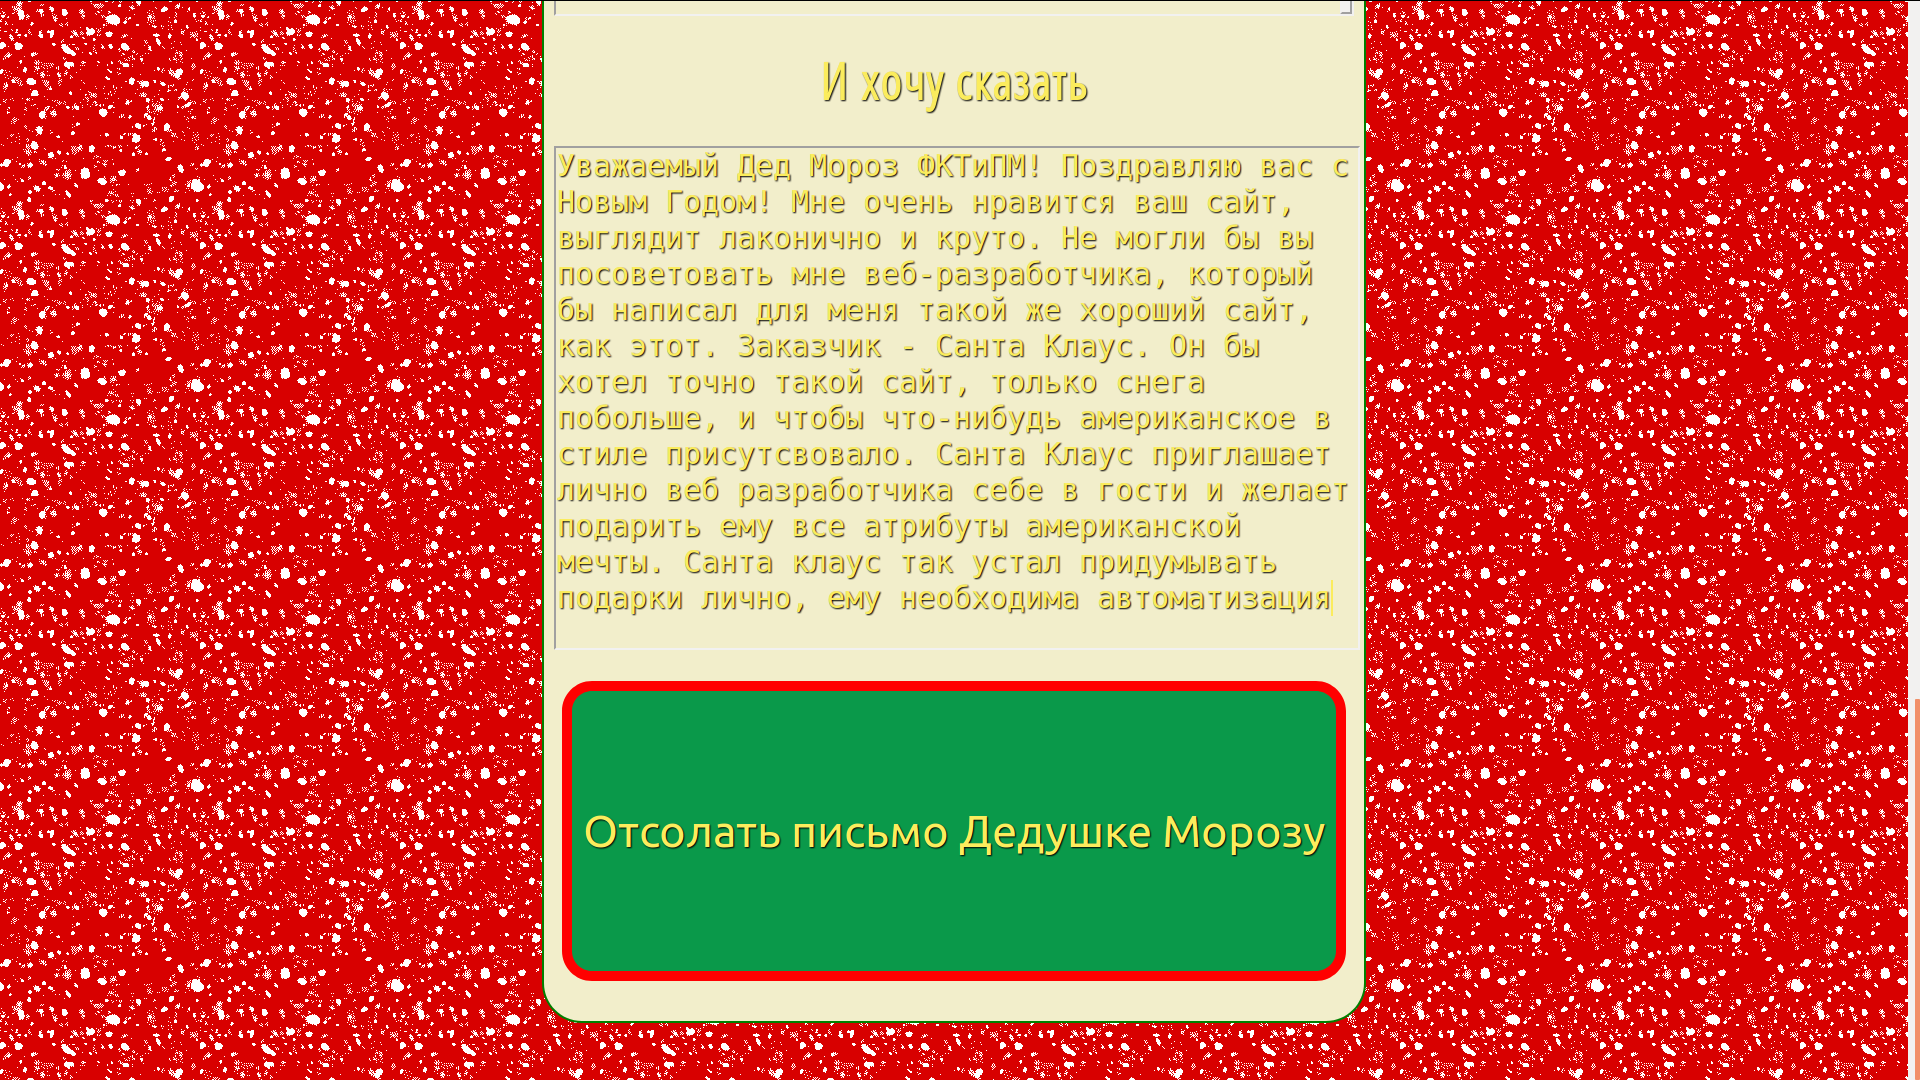
\includegraphics[width=\linewidth]{\picPath/text_and_button.png}
	\caption{ строка ввода поздравлений и кнопка }
  	\label{site:button}
\end{figure}

%Уважаемый Дед Мороз ФКТиПМ! Поздравляю вас с Новым Годом! Мне очень нравится ваш сайт, выглядит лаконично и круто. Не могли бы вы посоветовать мне веб-разработчика, который бы написал для меня такой же хороший сайт, как этот. Заказчик - Санта Клаус. Он бы хотел точно такой сайт, только снега побольше, и чтобы что-нибудь американское в стиле присутсвовало. Санта Клаус приглашает лично веб разработчика себе в гости и желает подарить ему все атрибуты американской мечты. Санта клаус так устал придумывать подарки лично, ему необходима автоматизация

На второй странице скрипт, написанный на javascript \cite{bib:js} выдает ответ в виде поздравлений и списка подарков. При этом вывод текста анимирован так, будто Дед Мороз сам пишет вам ответ(рисунок \ref{site:answer}). Это реализовано с помощью бесплатной  javascript библиотеки typed\_js \cite{bib:typed_js}. 

Задачи зачётной работы:
\begin{itemize}
\item  разработка сайта с использованием трехзвенной структуры;
\item разработка дизайна оформления, делающего сайт более привлекательным для пользователей;
\item  создание удобного интерфейса для возможности комфортного пребывания пользователей на сайте;
\end{itemize}    
   


\begin{figure}[H]
	\centering
	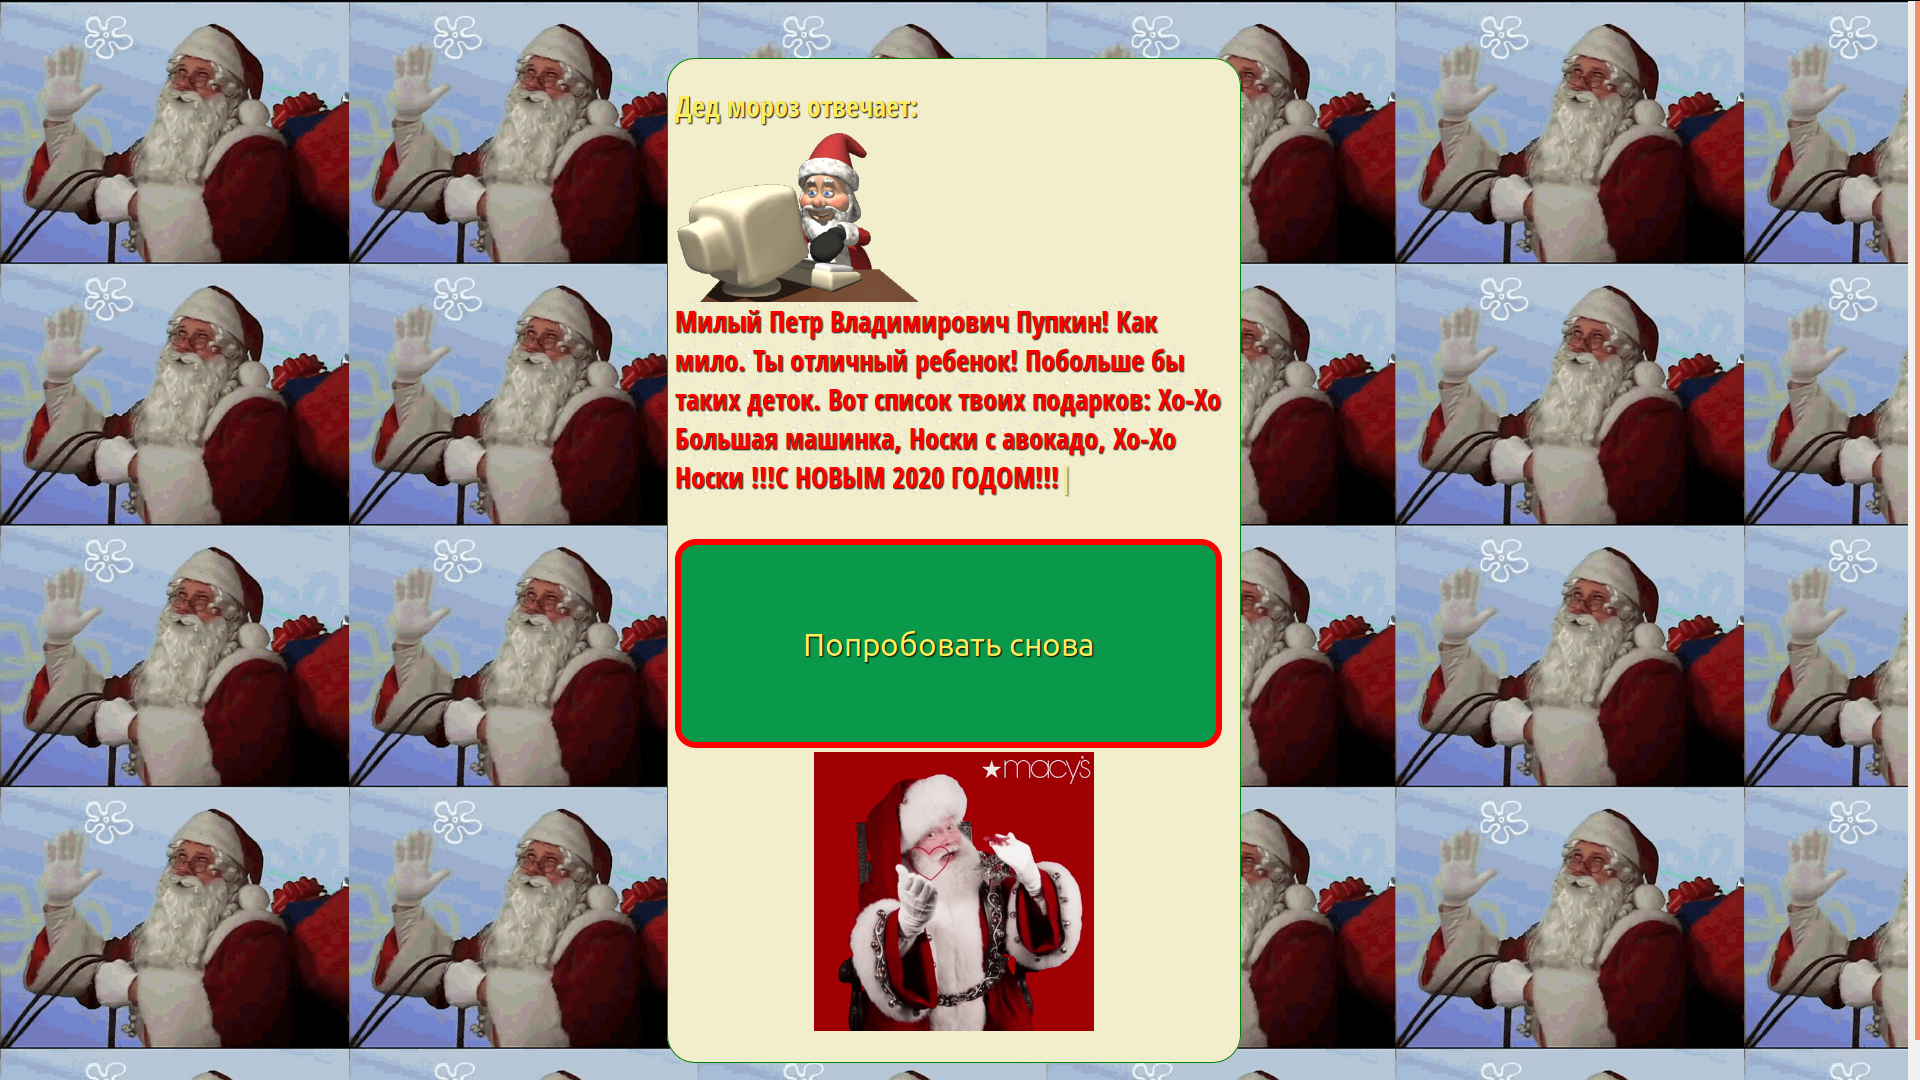
\includegraphics[width=\linewidth]{\picPath/answer.png}
	\caption{ строка ввода поздравлений и кнопка }
  	\label{site:answer}
\end{figure}

На первой странице пользователь выбирает десять пожеланий Деду Морозу. Каждое желание имеет свой вес, причем этот вес может быть как положительным, так и отрицательным. Каждый подарок, в свою очередь имеет свою цену, причем цена подарка тоже может быть отрицательной. Каждый пользователь после заполнения первой страницы получает счёт, равный сумме весов желаний, которые они выбрали. Подарки от Деда Мороза выдаются по следующему алгоритму:

\begin{enumerate}
\item если счет отрицательный, рассматривать только отрицательные подарки;
\item если счет положительный, рассматривать только положительные подарки;
\item если список возможных подарков пустой или счет нулевой - конец;
\item из списка допустимых подарков выбрать случайный;
\item если модуль счет не меньше, чем модуль цены этого подарка:
\begin{enumerate}
\item добавить подарок в список подарков;
\item уменьшить счет на цену подарка;
\end{enumerate}
\item иначе удалить из списка возможных подарков;
\item перейти на шаг 3
\end{enumerate}

В зависимости от счета пользователя, ему предлагается особенный стиль. Если, например, количество очков лежит в пределах от 0 до 	20, то пользователю будет предложен стиль, в котором Дедушка Мороз его благодарит. Если же, например, количество очков меньше -50 - то пользователю предлагается агрессивный дизайн. 

\section{Клиент-сервер}

Клиент – сервер процесс описывает взаимодействие между двумя компьютерными программами, при котором ода программа (клиент) направляет запрос к другой программе (серверу), которая выполняет данный запрос. Как правило, несколько клиентских программ обращаются к одной общей серверной программе. Например, веб-браузер – это клиентская программа, обращающаяся с запросами (на отправку веб страницы или файлов) к веб-серверу.
В моей работе сервером является приложение Apache, в нем хранится СУБД, к которому обращается клиентская часть.
Примером работы клиент-сервера является выдача подарков в соответствии с пожеланиями ребенка.



Back-end сайта реализован на языке php \cite{bib:php}, используя СУБД Mysql. Веб сервером выступает популярный для  php приложений Apache. В целом в реализации сайта Деда Мороза был использован стек технологий под названием LAMP (Linux,Apache,Mysql,PHP) Для реализации функционала сайта спроектирована база данный структуры, изображенной на \ref{bd}.
\chapter{Структура базы данных}

База данный реализована с помощью СУБД Mysql, её структуру можно наблюдать на рисунке \ref{bd}.

\begin{figure}[H]
\centering
	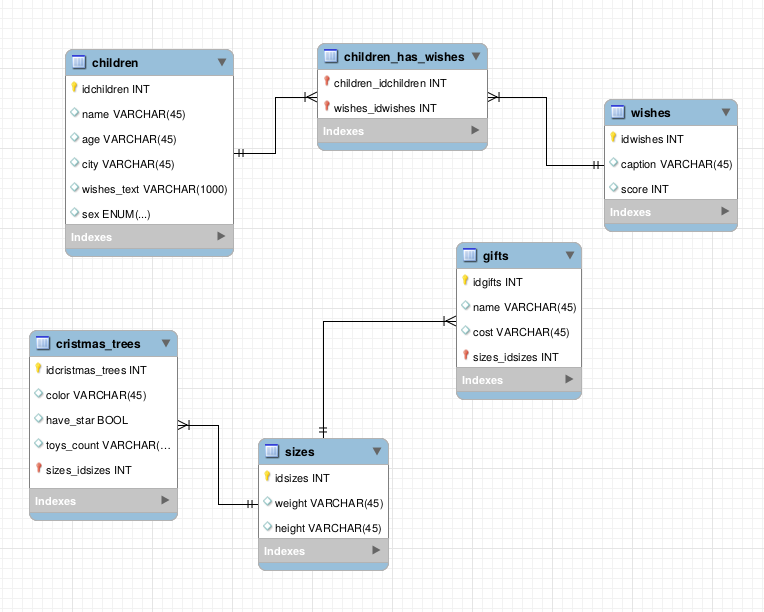
\includegraphics[width=\linewidth]{\picPath/bd.png}
	\caption{ структура базы данных }
  	\label{bd}

\end{figure}

На стороне сервера реализованы две процедуры обращения к базе данных: 
\begin{enumerate}
\item вставка в базу данных информации о ребенке; 
\item выбока пожеланий текущего ребенка, счет количества его очков и выборка подарков по алгоритму, описанному выше.
\end{enumerate}

Можно видеть пример запроса к базе данных из php на рисунке \ref{screnshot}

\begin{figure}[H]
\centering
	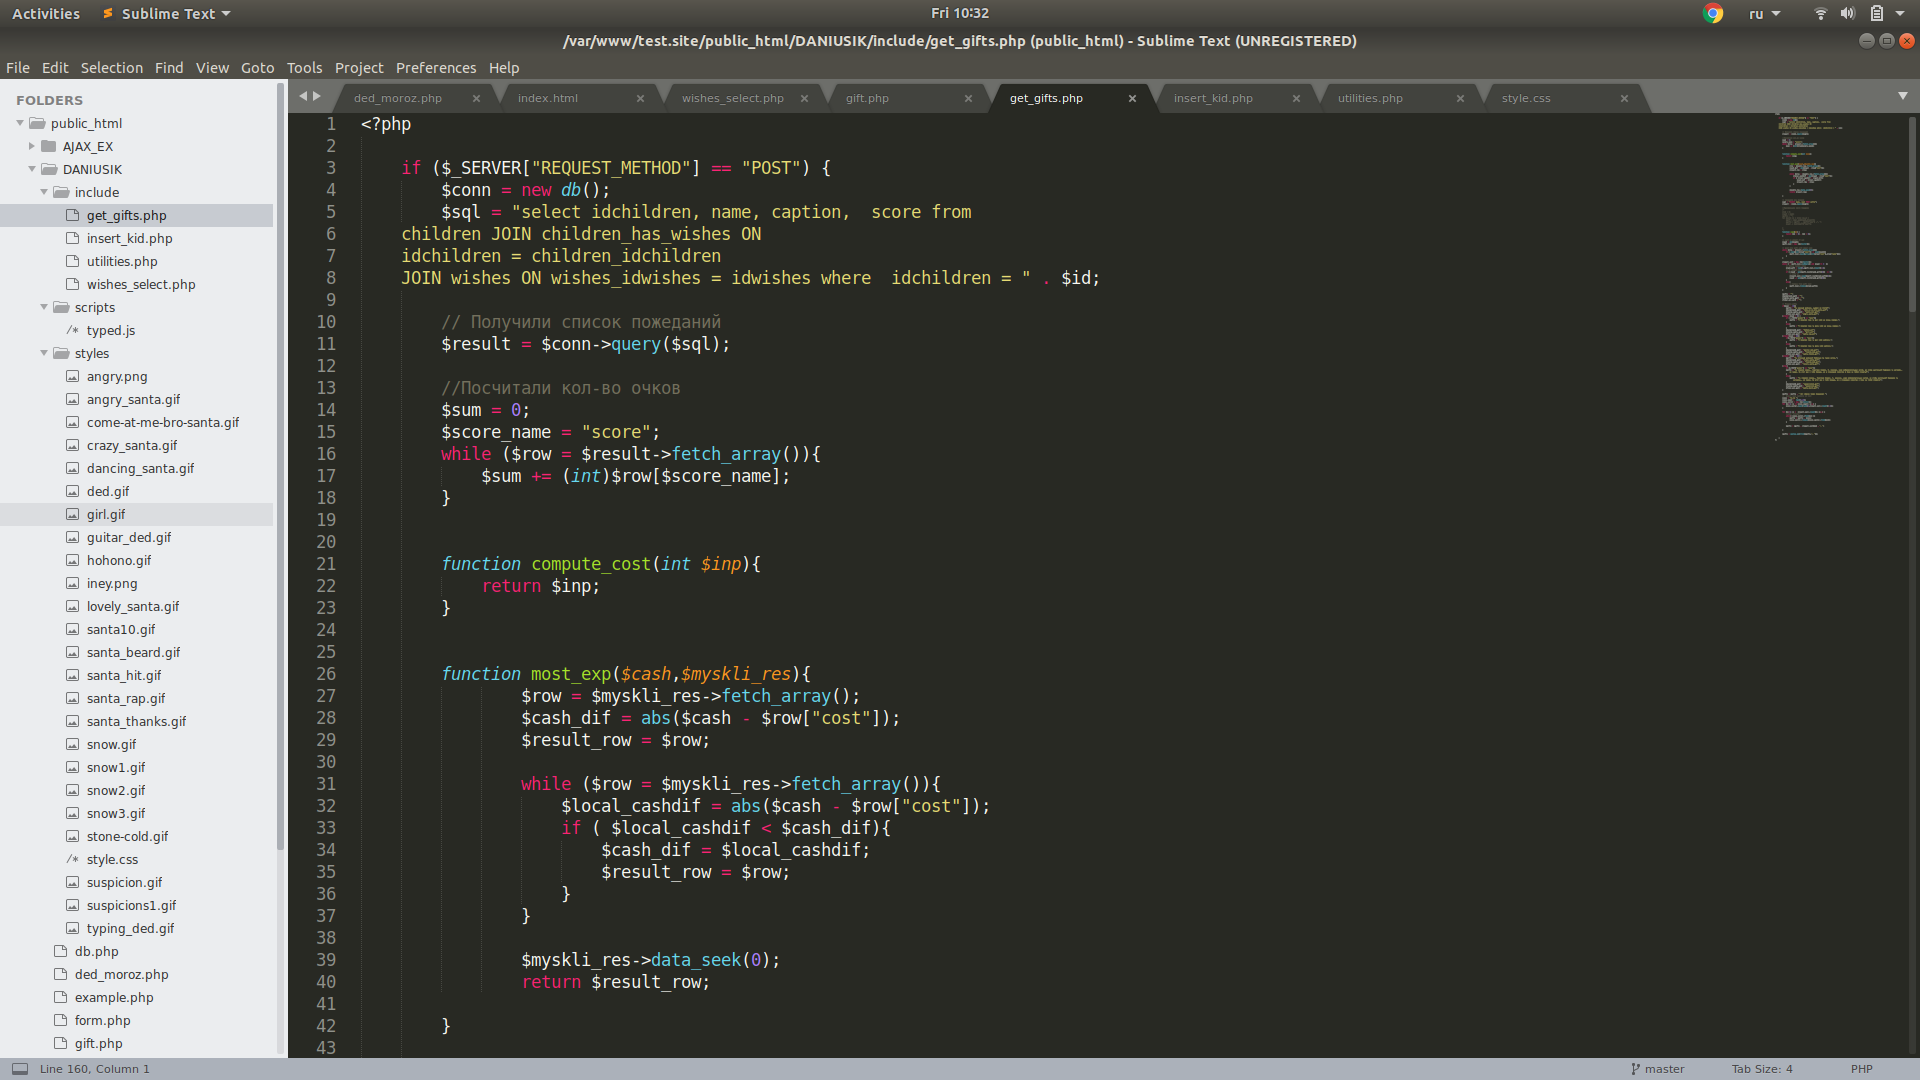
\includegraphics[width=\linewidth]{\picPath/screnshot.png}
	\caption{ пример запроса к базе данных }
  	\label{screnshot}

\end{figure}

\chapter{Код сайта}

Код сайта весьма сложен и длинен, поэтому в рамках отчета, его не удастся рассмотреть во всей полноте, однако можно привести важный составляющее его.

\section{Главная страница}

\begin{verbatim}
<!DOCTYPE html>
<html>
<html>
	<head>
			<meta charset="utf-8">
			<link href="https://fonts.googleapis.com/css?family=
			Open+Sans+Condensed:300" rel="stylesheet">
			<link href="styles/style.css" rel="stylesheet" type="text/css">
			<title>
				Пожелания для Деда Мороза
			</title>	
	</head>
<header>
	<div class=site_header>
	Официальный сайт Дедушки Мороза ФКТиПМ
	</div>
</header>	
<body>

<form action="gift.php" method="post">
	<h1>Дорогой Дедушка Мороз!</h1>
	<input type="hidden" name="example" value="data1">
	<h2>Меня зовут</h2>
	<input name="name" type="text" required><br>
	<h2>Мне уже исполнилось</h2>
	<input name="age" type="number" min="0" required><br>
	<h2>Я из города</h2>
	<input name="city" type="text" required><br>
	<h2>
  	<input type="radio" name="gender" value="male" checked> 
  	Мальчик<br>
 	<input type="radio" name="gender" value="female"> Девочка<br>
	</h2>

	<h1>Желаю тебе, Дедушка Мороз:</h1>

	<?php include 'include/wishes_select.php';?>
	<h1>И хочу сказать</h1>
	<textarea name="message" rows="1">С Новым Годом!</textarea>
	<br>
	<h1>
	<input type="submit"  value="Отослать письмо Дедушке Морозу"/> 
	</h1>
</form>
</body>
</html>
\end{verbatim}

\section{Процедура выдачи подарков}
\begin{verbatim}

		// push only gift with equal sign
		while ($row = $result->fetch_array()){
			if ( sign((int)$row['cost']) == sign($sum)){
				$gift_list->push(array((int)$row['cost'],$row['name']));
			}
		}

		$result_vect = new \Ds\Vector();
		while ( ! $gift_list->isEmpty() and $cash != 0  ){
			// Choose random index
			$rand_gift = rand(0,$gift_list->count()-1);
			// If enough money
			if ( $cash - abs($gift_list[$rand_gift][0])  >= 0){
				// Gift it
				$result_vect->push($gift_list[$rand_gift][1]);
				$cash -= abs($gift_list[$rand_gift][0]);
			}
			else{
				// Remove from gift list
				$gift_list->remove($rand_gift);
			}
		}
		
		$gifts = $gifts . " Вот список твоих подарков: ";
		//  Insert xoxo randomly in text
		$xoxo = "Хо-Хо ";
		$xoxo_count =  rand(3,10);
		$xoxo_vector = new \Ds\Vector();
		for ($i=0; $i <= $xoxo_count; $i++) { 
			$xoxo_vector->push(rand(0,$result_vect->count()-1));
		}

		for ($i=0; $i <  $result_vect->count(); $i++) { 
			//echo "string";
			while( $xoxo_vector->find($i) ){
				$gifts = $gifts . $xoxo;
				$xoxo_vector->remove($xoxo_vector->find($i));
			}

			$gifts = $gifts . $result_vect[$i] . ", ";
			
		}

		$gifts = quotes_js(rtrim($gifts,", "));

\end{verbatim}
\newpage
\begin{center}
\bfseries ЗАКЛЮЧЕНИЕ
\end{center}
\addcontentsline{toc}{chapter}{Заключение}

В рамках зачётной работы были рассмотрены основные методы проектировки и написания сайтов сети Интернет. В результате для рассматриваемых правил был разработан сайт на основе трёх звеньев (клиент – сервер – база данных) Деда Мороза ФКТиПМ. Сайт записывает информацию о всех пользователях, поддерживает интерактивное общение с пользователями благодаря библиотеке typed\_js.

Были изучены основные технологии создания веб приложений - серверный язык php, язык разметки css и браузерный язык javascript. Кроме того, изучены основы администрирования сайтов на примере популярного веб сервера Apache на платформе Linux. Рассмотрены возможности использования баз данных на примере СУБД Mysql.

\newpage
%список литературы
\addcontentsline{toc}{chapter}{Список использованных источников}

\begin{thebibliography}{0}

\bibitem{bib:meth} Архитектура «клиент-сервер» | Сетевые технологии / (Рус.). \urlTitle \url{http://www.4stud.info/networking/lecture5.html } [25 мая 2019]

\bibitem{bib:Sinica}Синица, С. Г. Веб-программирование и веб-сервисы : учебное пособие / С. Г. Синица ; М-во образования и науки Рос. Федерации, Кубанский гос. Ун-т. - Краснодар : [Кубанский государственный университет], 2013. - 158 с. 

\bibitem{bib:typed_js} Библиотека анимации текста type\_js / (Eng) \urlTitle \url{https://mattboldt.com/demos/typed-js}  [25 мая 2019]

\bibitem{bib:php} Онлайн учебник по изучению серверного языка программирования php / (Eng) \urlTitle \url{https://www.w3schools.com/php/}  
[25 мая 2019]

\bibitem{bib:html} Онлайн учебник по изучению языка разметки html / (Eng) \urlTitle \url{https://www.w3schools.com/html/} [25 мая 2019]


\bibitem{bib:css} Онлайн учебник по изучению языка стилей css / (Eng) \urlTitle \url{https://www.w3schools.com/css/} [25 мая 2019]

\bibitem{bib:js} Онлайн учебник по изучению браузерного языка javascript / (Eng) \urlTitle \url{https://www.w3schools.com/js/} [25 мая 2019]

\bibitem{bib:habr} Почему не стоит использовать двухуровневую архитектуру при разработке клиент-серверных приложений / (Ru) \urlTitle \url{https://habr.com/ru/post/348946/} [25 мая 2019]

\end{thebibliography}
\end{document}